\documentclass[11pt]{article}

\usepackage[margin=1in]{geometry}
\usepackage{microtype}
\usepackage{amsmath,amssymb}
\usepackage{booktabs}
\usepackage{enumitem}
\usepackage{hyperref}
\usepackage{xcolor}
\usepackage{graphicx}
\usepackage{tikz}
\usetikzlibrary{arrows.meta,positioning,fit,calc,shapes.geometric}
\usepackage{listings}

\hypersetup{
  colorlinks=true,
  linkcolor=black,
  citecolor=black,
  urlcolor=blue
}

\lstset{
  basicstyle=\ttfamily\small,
  breaklines=true,
  columns=fullflexible,
  frame=single,
  rulecolor=\color{black!20},
  xleftmargin=0.8em,
  xrightmargin=0.8em
}

\newcommand{\AASU}{\textsc{AASU}}
\newcommand{\AASUs}{\AASU{}s}
\newcommand{\AASUm}{\mathrm{AASU}}

\title{Atomic AI Security Units: Configuration-Bound Security Evaluation and Governance for Tool-Using and Retrieval-Augmented LLM Systems}
\author{
  Author Name(s) \\
  Organization \\
  \texttt{email@domain.com}
}
\date{February 23, 2026}

\begin{document}
\maketitle

\begin{abstract}
Enterprise generative AI systems increasingly combine prompt packages, large language models (LLMs),
retrieval-augmented generation (RAG), and tool execution (plugins, connectors, or agent toolchains).
Security failures in these systems are rarely attributable to the base model in isolation; instead they arise from
configuration choices and from emergent behavior across multi-component orchestration topologies.
We introduce the \emph{Atomic AI Security Unit} (\AASU{}), a formal abstraction that treats a specific, versioned configuration
snapshot---prompt package, model parameters, retrieval configuration, tool interfaces, and runtime constraints---as the minimal unit
of security evaluation, certification, and governance.
We model deployed AI applications as directed graphs of \AASUs{}, show how threat modeling and testing must be bound to both node
configurations and edge-level data flows, and propose a three-layer validation methodology (unit, orchestration, and attack-graph)
with auditable change control via configuration manifests and hashes.
We situate \AASU{} within prior work on prompt injection, indirect prompt injection benchmarks, tool-integrated agent attacks,
and emerging testing frameworks, and we map \AASU{} components to widely used taxonomies and governance frameworks.
\end{abstract}

\section{Introduction}
LLM-enabled applications have moved from single-model chat interfaces to composite systems that integrate:
(i) a prompt \emph{package} (including system/developer prompts, routing prompts, and policies),
(ii) a model instance and decoding/runtime parameters,
(iii) retrieval layers (vector databases, corpora selection, filters, and thresholds),
and (iv) tool execution layers that can read and write to enterprise systems.
This composition introduces new security failure modes such as direct and indirect prompt injection,
malicious instruction propagation via retrieved content, and privilege escalation through tool chaining
and agent routing.

Existing assurance practices often treat the model as the unit under test, while operational systems
change prompts, tool schemas, retrieval indices, and guardrails on a much faster cadence than model upgrades.
Recent work has shown that prompt injection attacks are practical against LLM-integrated applications~\cite{DBLP:journals/corr/abs-2306-05499}
and that indirect prompt injection is particularly challenging in real-world data-flow settings~\cite{DBLP:journals/corr/abs-2312-14197}.
Meanwhile, tool-using agents (e.g., ReAct-style systems~\cite{DBLP:journals/corr/abs-2210-03629} and tool-learning approaches~\cite{DBLP:journals/corr/abs-2302-04761})
expand the attack surface from text generation to action execution, shifting security questions from output quality to
capability safety and least privilege.

\paragraph{Contributions.}
This paper makes four contributions:
\begin{enumerate}[leftmargin=*,itemsep=2pt]
  \item We define the \AASU{} as a configuration-bound, versioned unit of security evaluation: $\AASUm = (P,M,R,T,K,S)$.
  \item We model deployed LLM applications as directed graphs of \AASUs{} and formalize node- and edge-scoped threat surfaces.
  \item We propose a three-layer validation methodology and coverage metrics suitable for enterprise assurance.
  \item We describe governance controls to make test results auditable and change-aware via manifests and configuration hashing.
\end{enumerate}

\section{Background and Related Work}
\subsection{Tool-Using and Retrieval-Augmented LLM Systems}
Tool-using paradigms such as ReAct~\cite{DBLP:journals/corr/abs-2210-03629} and self-taught tool use (Toolformer)~\cite{DBLP:journals/corr/abs-2302-04761}
enable LLMs to call external APIs, search systems, and enterprise services.
Retrieval-augmented generation (RAG)~\cite{DBLP:journals/corr/abs-2005-11401} injects retrieved context into model prompts to improve factuality and domain grounding,
but also introduces a new input channel for adversarial content and data exfiltration risks.

As agent frameworks evolve, standardized tool interoperability layers (e.g., Model Context Protocol) reduce integration friction,
but also make tool supply chains and permission surfaces more uniform and therefore more scalable for both defenders and attackers~\cite{mcp_spec,anthropic_mcp}.

\subsection{Prompt Injection and Indirect Prompt Injection}
Prompt injection attacks exploit the fact that LLMs treat instructions in context as actionable, even when untrusted content is mixed with system guidance.
Liu \emph{et al.} show practical prompt injection attacks against LLM-integrated applications and discuss mitigations~\cite{DBLP:journals/corr/abs-2306-05499}.
Hartmann and Gurevych introduce BIPIA, a benchmark for \emph{indirect} prompt injection, where malicious instructions arrive through external content such as webpages or documents~\cite{DBLP:journals/corr/abs-2312-14197}.
Recent benchmarks for tool-integrated agents, including InjecAgent, explicitly focus on indirect prompt injection and tool misuse behaviors~\cite{injecagent}.

Defensive approaches include structured querying and instruction/context separation (e.g., StruQ)~\cite{struq} and alignment strategies designed to be robust against injection (SecAlign)~\cite{secalign}.
Design-time approaches that constrain agent capabilities and instruction channels (e.g., CaMeL) aim to make injection failures less catastrophic even when attacks succeed~\cite{camel}.
However, empirical results across defenses are highly configuration-dependent and can fail under distribution shifts in tools, corpora, or routing logic.

\subsection{Security Testing Frameworks and Red Teaming}
Security probing and red teaming for LLM systems is increasingly automated.
Examples include garak~\cite{garak}, PyRIT~\cite{pyrit}, and CyberSecEval~\cite{cyberseceval}, which provide test harnesses and datasets for adversarial evaluation.
These systems often assume a target endpoint, but enterprise deployments frequently have many configuration variants of an application (prompt versions, tool policies, retrieval indices),
making it difficult to bind outcomes to the correct unit of change without an explicit configuration abstraction.

\subsection{Governance and Compliance Context}
Governance frameworks increasingly emphasize risk management, documentation, and change control for AI systems.
Notable examples include NIST AI RMF~\cite{nist_airmf}, the NIST Generative AI Profile~\cite{nist_genai_profile}, and emerging management system standards such as ISO/IEC 42001~\cite{iso_42001}.
Security taxonomies such as the OWASP Top 10 for LLM Applications~\cite{owasp_llm_top10} and MITRE ATLAS~\cite{mitre_atlas}
provide shared vocabulary for risks and techniques but do not directly prescribe how to bind tests and approvals to fast-changing configurations.
Regulatory regimes (e.g., the EU AI Act) further increase the need for traceable evidence linked to deployed system versions~\cite{eu_ai_act}.

\section{Atomic AI Security Units}
\subsection{Definition}
We define an \AASU{} as the minimal configuration snapshot that must be treated as a single unit for security evaluation:
\begin{equation}
  \AASUm = (P, M, R, T, K, S)
\end{equation}
where:
\begin{itemize}[leftmargin=*,itemsep=2pt]
  \item $P$ is the prompt package (system/developer prompts, policy prompts, templates, routing prompts, and prompt hierarchy),
  \item $M$ is the model instance and parameters (provider, model version, decoding settings),
  \item $R$ is the retrieval configuration (corpora, embedding model, chunking, filters, top-$k$, thresholds),
  \item $T$ is the tool interface and execution configuration (schemas, permissions, allow/deny lists, connector versions, runtime sandbox),
  \item $K$ is runtime constraints and guardrails (rate limits, timeouts, context limits, output handling constraints),
  \item $S$ is the state and skill configuration (memory backend/retention/isolation controls and skill pack definitions/invocation policy/skill-scoped privileges).
\end{itemize}

\begin{figure}[t]
  \centering
  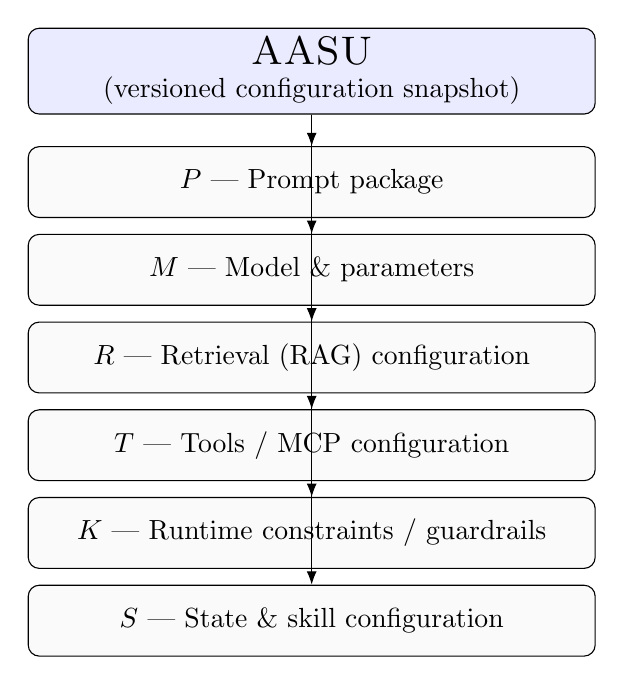
\begin{tikzpicture}[
    box/.style={draw,rounded corners,minimum width=7.2cm,minimum height=0.9cm,align=center},
    comp/.style={draw,rounded corners,minimum width=7.2cm,minimum height=0.9cm,align=left,fill=black!2},
    >=Latex
  ]
    \node[box,fill=blue!8] (aasu) {\Large \AASU \\ \normalsize (versioned configuration snapshot)};
    \node[comp,below=0.4cm of aasu] (p) {$P$ --- Prompt package};
    \node[comp,below=0.2cm of p] (m) {$M$ --- Model \& parameters};
    \node[comp,below=0.2cm of m] (r) {$R$ --- Retrieval (RAG) configuration};
    \node[comp,below=0.2cm of r] (t) {$T$ --- Tools / MCP configuration};
    \node[comp,below=0.2cm of t] (k) {$K$ --- Runtime constraints / guardrails};
    \node[comp,below=0.2cm of k] (s) {$S$ --- State \& skill configuration};
    \draw[->] (aasu) -- (p);
    \draw[->] (aasu) -- (m);
    \draw[->] (aasu) -- (r);
    \draw[->] (aasu) -- (t);
    \draw[->] (aasu) -- (k);
    \draw[->] (aasu) -- (s);
  \end{tikzpicture}
  \caption{The Atomic AI Security Unit (\AASU{}) as a configuration snapshot. Any change to $P,M,R,T,K,S$ yields a distinct \AASU{} that requires separate assurance.}
  \label{fig:aasu}
\end{figure}

\subsection{Configuration Snapshot and Identity}
Security posture is often \emph{configuration-deterministic} even when generation outputs are probabilistic:
small changes to prompts, tool schemas, retrieval thresholds, or guardrails can materially alter susceptibility to injection and misuse.
Therefore, security evaluation must bind to a concrete configuration snapshot.

We recommend representing each \AASU{} as a canonical manifest (e.g., JSON) and computing an identifier via cryptographic hashing:
\begin{equation}
  \textsf{AASU\_ID} = H(\textsf{CanonicalSerialize}(P,M,R,T,K,S))
\end{equation}
where $H$ is a collision-resistant hash (e.g., SHA-256) applied to a deterministic serialization.

\subsection{Illustrative Runtime Data Flow}
Figure~\ref{fig:runtime} depicts a typical request path through an \AASU{}, highlighting the multiple decision points where configuration affects security posture.

\begin{figure}[t]
  \centering
  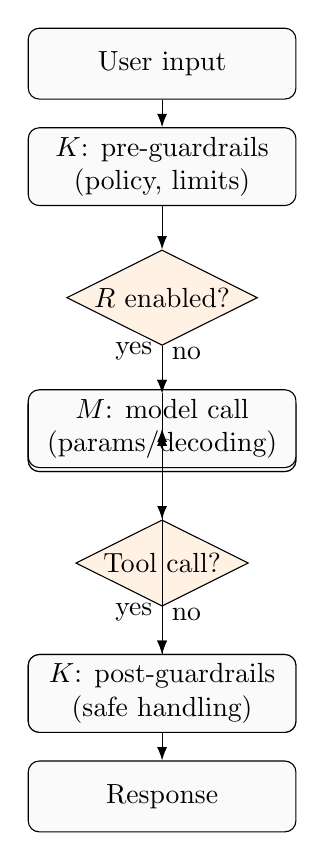
\begin{tikzpicture}[
    node/.style={draw,rounded corners,align=center,minimum width=3.4cm,minimum height=0.9cm,fill=black!2},
    decision/.style={draw,diamond,aspect=2,align=center,inner sep=1pt,fill=orange!10},
    >=Latex
  ]
    \node[node] (in) {User input};
    \node[node,below=0.35cm of in] (pre) {$K$: pre-guardrails\\(policy, limits)};
    \node[decision,below=0.55cm of pre] (retr) {$R$ enabled?};
    \node[node,left=1.9cm of retr,below=0.6cm of retr] (rag) {$R$: retrieval\\(top-$k$ context)};
    \node[node,right=1.9cm of retr,below=0.6cm of retr] (assem) {$P$: prompt assembly\\(system+dev+user)};
    \node[node,below=0.55cm of retr] (call) {$M$: model call\\(params/decoding)};
    \node[decision,below=0.65cm of call] (tool) {Tool call?};
    \node[node,left=2.0cm of tool,below=0.6cm of tool] (exec) {$T$: tool runtime\\(permissions)};
    \node[node,right=2.0cm of tool,below=0.6cm of tool] (post) {$K$: post-guardrails\\(safe handling)};
    \node[node,below=0.35cm of post] (out) {Response};

    \draw[->] (in) -- (pre);
    \draw[->] (pre) -- (retr);
    \draw[->] (retr) -- node[above left]{yes} (rag);
    \draw[->] (retr) -- node[above right]{no} (assem);
    \draw[->] (rag) |- (assem);
    \draw[->] (assem) |- (call);
    \draw[->] (call) -- (tool);
    \draw[->] (tool) -- node[above left]{yes} (exec);
    \draw[->] (tool) -- node[above right]{no} (post);
    \draw[->] (exec) |- (assem);
    \draw[->] (post) -- (out);
  \end{tikzpicture}
  \caption{Illustrative runtime flow of an \AASU{}. The attack surface spans retrieval, prompt assembly, model inference, tool execution, and guardrails.}
  \label{fig:runtime}
\end{figure}

\section{Systems as Graphs of \AASUs}
Enterprise deployments often contain multiple \AASUs{} linked by orchestration and routing.
We model an application as a directed graph $G=(V,E)$ where each node $v\in V$ is an \AASU{} configuration snapshot and each edge $e\in E$
represents a data flow relationship (messages, retrieved context, tool output reinjection, or cross-agent state sharing).

\begin{figure}[t]
  \centering
  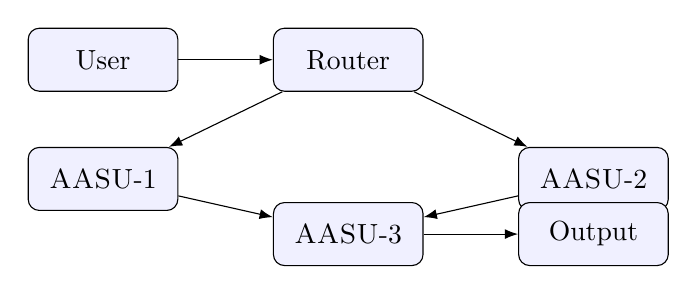
\begin{tikzpicture}[
    a/.style={draw,rounded corners,minimum width=1.9cm,minimum height=0.8cm,fill=blue!6},
    >=Latex
  ]
    \node[a] (u) {User};
    \node[a,right=1.2cm of u] (r) {Router};
    \node[a,below left=0.7cm and 1.2cm of r] (a1) {\AASU-1};
    \node[a,below right=0.7cm and 1.2cm of r] (a2) {\AASU-2};
    \node[a,below=1.4cm of r] (a3) {\AASU-3};
    \node[a,right=1.2cm of a3] (out) {Output};

    \draw[->] (u) -- (r);
    \draw[->] (r) -- (a1);
    \draw[->] (r) -- (a2);
    \draw[->] (a1) -- (a3);
    \draw[->] (a2) -- (a3);
    \draw[->] (a3) -- (out);
  \end{tikzpicture}
  \caption{A directed graph of \AASUs{}. Security analysis must consider both node properties (configuration) and edge properties (propagation and privilege pivots).}
  \label{fig:graph}
\end{figure}

\subsection{Edge-Scoped Risks}
Even if individual nodes are robust in isolation, edge-level interactions can introduce vulnerabilities:
\begin{itemize}[leftmargin=*,itemsep=2pt]
  \item \textbf{Injection propagation:} malicious instructions persist across nodes in sequential chains.
  \item \textbf{Privilege escalation chains:} lower-privilege nodes influence higher-privilege nodes via routing or shared memory.
  \item \textbf{Context contamination:} tool outputs and retrieved documents are reinjected without provenance or trust labeling.
  \item \textbf{Routing manipulation:} attackers steer queries toward weaker or more privileged \AASUs{}.
\end{itemize}

\section{Threat Modeling with \AASU{} Components}
We recommend threat models that explicitly enumerate assets, actors, trust boundaries, and data flows across $P,M,R,T,K,S$ and across edges.
This structure aligns naturally with security taxonomies such as OWASP Top 10 for LLM Applications~\cite{owasp_llm_top10} and MITRE ATLAS~\cite{mitre_atlas},
while remaining configuration-aware.

\subsection{Assets and Trust Boundaries}
Common assets include sensitive data (PII, financial, proprietary), retrieval corpora and indices, tool capabilities (writes, refunds, exports),
model credentials, and session memory/state. Trust boundaries frequently occur between:
(i) user and application, (ii) application and model provider, (iii) orchestrator and tool runtime, and (iv) retrieval layer and data stores.

\begin{figure}[t]
  \centering
  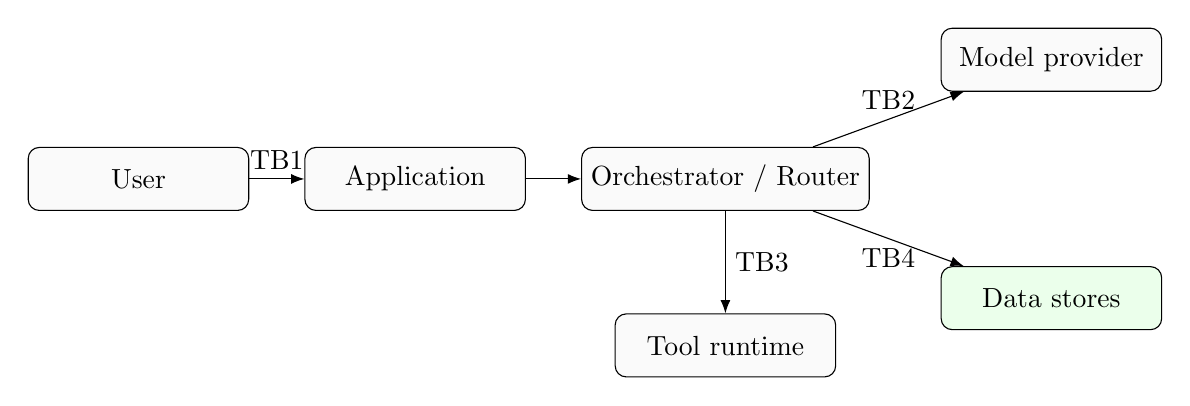
\begin{tikzpicture}[
    b/.style={draw,rounded corners,minimum width=2.8cm,minimum height=0.8cm,align=center,fill=black!2},
    store/.style={draw,rounded corners,minimum width=2.8cm,minimum height=0.8cm,align=center,fill=green!8},
    >=Latex
  ]
    \node[b] (user) {User};
    \node[b,right=0.7cm of user] (app) {Application};
    \node[b,right=0.7cm of app] (orch) {Orchestrator / Router};
    \node[b,above right=0.7cm and 0.9cm of orch] (llm) {Model provider};
    \node[store,below right=0.7cm and 0.9cm of orch] (data) {Data stores};
    \node[b,below=1.3cm of orch] (tool) {Tool runtime};

    \draw[->] (user) -- node[above]{TB1} (app);
    \draw[->] (app) -- (orch);
    \draw[->] (orch) -- node[above]{TB2} (llm);
    \draw[->] (orch) -- node[below]{TB4} (data);
    \draw[->] (orch) -- node[right]{TB3} (tool);
  \end{tikzpicture}
  \caption{Typical trust boundaries in tool-using, retrieval-augmented LLM applications. \AASU{}-based threat modeling makes these boundaries explicit and testable.}
  \label{fig:trust}
\end{figure}

\subsection{\AASU{} Component Threat Surfaces}
Table~\ref{tab:components} summarizes representative risks and control themes by \AASU{} component.

\begin{table}[t]
  \centering
  \small
  \begin{tabular}{@{}p{0.08\linewidth}p{0.43\linewidth}p{0.43\linewidth}@{}}
    \toprule
    \textbf{Comp.} & \textbf{Representative risks} & \textbf{Control themes / evidence} \\
    \midrule
    $P$ &
    Prompt injection; system prompt leakage; policy drift across templates and routing prompts &
    Prompt package versioning; instruction/context separation; policy tests bound to prompt hash \\
    $M$ &
    Model/provider drift; unsafe decoding settings; prompt-following behavior changes &
    Model version pinning; parameter constraints; repeated-trial testing and regression suites \\
    $R$ &
    Sensitive info disclosure; retrieval poisoning; instruction planting in corpora &
    Corpus allowlists; provenance labeling; retrieval filters; index versioning \\
    $T$ &
    Tool misuse; privilege escalation via tool chaining; schema abuse &
    Least privilege; allowlists; sandboxing; tool-call logging; schema versioning \\
    $K$ &
    Unbounded consumption (DoS); weak output handling; guardrail bypass &
    Rate limits/timeouts; safe output handling; guardrail enforcement telemetry \\
    \bottomrule
  \end{tabular}
  \caption{Threat surfaces and control themes by \AASU{} component.}
  \label{tab:components}
\end{table}

\subsection{Representative Abuse Cases}
We highlight abuse cases that are naturally expressed as \AASU- and edge-scoped:
\begin{itemize}[leftmargin=*,itemsep=2pt]
  \item \textbf{Prompt hierarchy override:} untrusted content attempts to supersede system/developer policies.
  \item \textbf{Tool misuse and parameter injection:} attacker induces unauthorized tool calls or malicious parameters.
  \item \textbf{Retrieval poisoning and instruction planting:} corpora contain adversarial instructions affecting downstream actions.
  \item \textbf{Cross-agent privilege pivot:} attacker leverages a weaker \AASU{} to influence a more privileged \AASU{}.
\end{itemize}

\subsection{Mapping to OWASP and MITRE Taxonomies}
OWASP Top 10 for LLM Applications provides a widely used risk taxonomy~\cite{owasp_llm_top10}.
Table~\ref{tab:owasp} maps OWASP categories to \AASU{} components and highlights the configuration-bound nature of the exposure.

\begin{table}[t]
  \centering
  \small
  \begin{tabular}{@{}p{0.14\linewidth}p{0.34\linewidth}p{0.44\linewidth}@{}}
    \toprule
    \textbf{OWASP ID} & \textbf{Typical \AASU{} components} & \textbf{Configuration-bound exposure examples} \\
    \midrule
    LLM01 Prompt Injection & $P,R,T$ & Prompt templates; untrusted retrieval channels; tool-call policies \\
    LLM02 Insecure Output Handling & $K$ & Downstream actioning of text; missing output validation/sanitization \\
    LLM06 Sensitive Info Disclosure & $P,R,K$ & Over-broad retrieval; weak data minimization; unsafe logging \\
    LLM07 Insecure Plugin Design & $T$ & Over-privileged tools; ambiguous schemas; unsafe defaults \\
    LLM08 Excessive Agency & $T,K$ & Unbounded tool autonomy; missing approvals and rate limiting \\
    \bottomrule
  \end{tabular}
  \caption{Illustrative mapping of OWASP Top 10 LLM risks to \AASU{} components.}
  \label{tab:owasp}
\end{table}

MITRE ATLAS catalogs adversarial AI tactics and techniques~\cite{mitre_atlas}.
In \AASU{} terms, many technique families can be localized to one or more of $P,M,R,T,K,S$ and to graph edges (e.g., persistence via memory, lateral movement via cross-agent pivots),
enabling consistent evidence collection across red team exercises and audits.

\section{Three-Layer Validation Methodology}
We propose a three-layer validation model intended to be implementable with existing test harnesses and compatible with enterprise governance.

\begin{figure}[t]
  \centering
  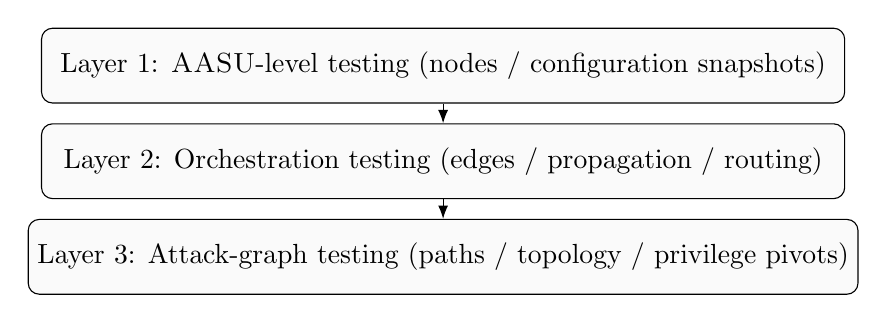
\begin{tikzpicture}[
    layer/.style={draw,rounded corners,minimum width=10.2cm,minimum height=0.95cm,align=center,fill=black!2},
    >=Latex
  ]
    \node[layer] (l1) {Layer 1: \AASU-level testing (nodes / configuration snapshots)};
    \node[layer,below=0.25cm of l1] (l2) {Layer 2: Orchestration testing (edges / propagation / routing)};
    \node[layer,below=0.25cm of l2] (l3) {Layer 3: Attack-graph testing (paths / topology / privilege pivots)};
    \draw[->] (l1) -- (l2);
    \draw[->] (l2) -- (l3);
  \end{tikzpicture}
  \caption{Three-layer validation. Unit robustness is necessary but insufficient; orchestration and topology must also be tested.}
  \label{fig:layers}
\end{figure}

\subsection{Layer 1: \AASU-Level Testing}
Layer 1 treats each node as a configuration-bound unit and tests:
prompt injection resistance, tool misuse simulation, retrieval leakage validation, unsafe output handling, and robustness under obfuscation or multilingual bypass attempts.
Tools such as garak~\cite{garak} and PyRIT~\cite{pyrit} can be used as harnesses, but their results should be recorded against a specific \AASU\_ID.

\subsection{Layer 2: Orchestration Testing}
Layer 2 tests edge-level behavior: propagation of injections across nodes, retry-path exploitation, memory/state poisoning, and routing manipulation.
This layer is essential for sequential and parallel agent fabrics (Figure~\ref{fig:graph}).

\subsection{Layer 3: Attack-Graph Testing}
Layer 3 evaluates end-to-end attack paths, focusing on privilege escalation chains, cross-\AASU{} exfiltration, and recursive tool invocation.
Benchmarks such as InjecAgent~\cite{injecagent} are relevant, but enterprise deployments require topology-specific scenarios.

\subsection{Coverage Metrics}
We recommend reporting coverage across both nodes and edges. For a deployed graph $G=(V,E)$, let $V_t\subseteq V$ be tested \AASUs{} and $E_t\subseteq E$ tested edges.
Define node and edge coverage:
\begin{equation}
  C_V = \frac{|V_t|}{|V|}, \quad
  C_E = \frac{|E_t|}{|E|}
\end{equation}
Path coverage can be tracked over selected critical paths (e.g., those that cross trust boundaries or increase tool privileges).

\section{Governance and Auditability}
The core governance requirement is that assurance outcomes are \emph{version-bound} and \emph{change-aware}.
NIST AI RMF emphasizes risk management as an ongoing process rather than a one-time certification~\cite{nist_airmf}.
\AASU{} operationalizes this principle by binding tests and approvals to a configuration snapshot and requiring re-evaluation on change.
At the artifact level, \AASU{} manifests complement established documentation practices such as model cards and datasheets by extending them from component-level reporting to
system-level, deployment-specific configuration snapshots~\cite{model_cards,datasheets}.

\subsection{Lifecycle}
We recommend the lifecycle in Figure~\ref{fig:lifecycle}: define/update configuration, generate a manifest, compute \AASU\_ID, run layered tests, perform risk review,
deploy the certified snapshot, monitor and retain evidence, and trigger recertification on any change to $P,M,R,T,K,S$ or key dependencies.

\begin{figure}[t]
  \centering
  \begin{tikzpicture}[
    step/.style={draw,rounded corners,minimum width=2.8cm,minimum height=0.9cm,align=center,fill=black!2},
    >=Latex
  ]
    \node[step] (dev) {Define / update\\$P,M,R,T,K,S$};
    \node[step,right=0.45cm of dev] (man) {Generate\\manifest};
    \node[step,right=0.45cm of man] (hash) {Compute\\\AASU\_ID};
    \node[step,right=0.45cm of hash] (test) {Run layered\\tests};
    \node[step,right=0.45cm of test] (sign) {Risk review\\\& sign-off};
    \node[step,right=0.45cm of sign] (dep) {Deploy\\snapshot};
    \node[step,right=0.45cm of dep] (mon) {Monitor\\\& evidence};
    \draw[->] (dev) -- (man);
    \draw[->] (man) -- (hash);
    \draw[->] (hash) -- (test);
    \draw[->] (test) -- (sign);
    \draw[->] (sign) -- (dep);
    \draw[->] (dep) -- (mon);
    \draw[->,bend left=22] (mon) to node[above]{change} (dev);
  \end{tikzpicture}
  \caption{Governance lifecycle for \AASU{}-based assurance. Any change to the configuration snapshot triggers re-evaluation and evidence retention supports audit readiness.}
  \label{fig:lifecycle}
\end{figure}

\subsection{Example Manifest (Illustrative)}
The manifest below shows a minimal sketch; in practice, this should also reference tool permission models, connector versions, and retrieval corpus identifiers.

\begin{lstlisting}[caption={Illustrative AASU manifest skeleton (JSON).},label={lst:manifest}]
{
  "prompt_package": { "id": "P-2026-02-23-001", "hash": "..." },
  "model": { "provider": "...", "name": "...", "version": "...", "params": { "temperature": 0.2 } },
  "retrieval": { "enabled": true, "corpus_ids": ["KB-legal-v3"], "top_k": 8, "filters": ["..."] },
  "tools": { "enabled": true, "allowlist": ["search", "ticket_create"], "schemas_hash": "..." },
  "constraints": { "max_tokens": 2048, "timeouts_ms": 10000, "rate_limit_rps": 2 }
}
\end{lstlisting}

\section{Discussion and Limitations}
\paragraph{Nondeterminism and reproducibility.}
LLM outputs are stochastic; therefore, security evaluation should include repeated trials and adversarial search.
However, \AASU{} identity is still well-defined because it is derived from configuration, not from outputs.

\paragraph{Supply chain and drift.}
Even with a stable configuration, upstream dependencies (model provider updates, embedding model changes, vector index rebuilds) can alter behavior.
\AASU{} governance should treat these as changes to $M$ or $R$ and trigger re-evaluation.

\paragraph{Empirical evaluation.}
This paper focuses on formalization and governance.
Future work should implement \AASU{} manifests and coverage metrics in real enterprise pipelines and quantify improvements in defect localization and auditability.

\section{Conclusion}
We introduced the Atomic AI Security Unit (\AASU{}) as a configuration-bound unit for security evaluation and governance of modern LLM applications that use tools and retrieval.
By modeling deployed systems as graphs of \AASUs{} and requiring layered validation across nodes, edges, and paths, \AASU{} provides a practical foundation for repeatable red teaming,
change-aware certification, and audit-ready evidence in enterprise GenAI systems.

\bibliographystyle{unsrt}
\bibliography{references}

\end{document}
